% Chapter 1

\chapter{Preliminaries}\label{ch:Basis}

\begin{figure}[t]
    \centering
    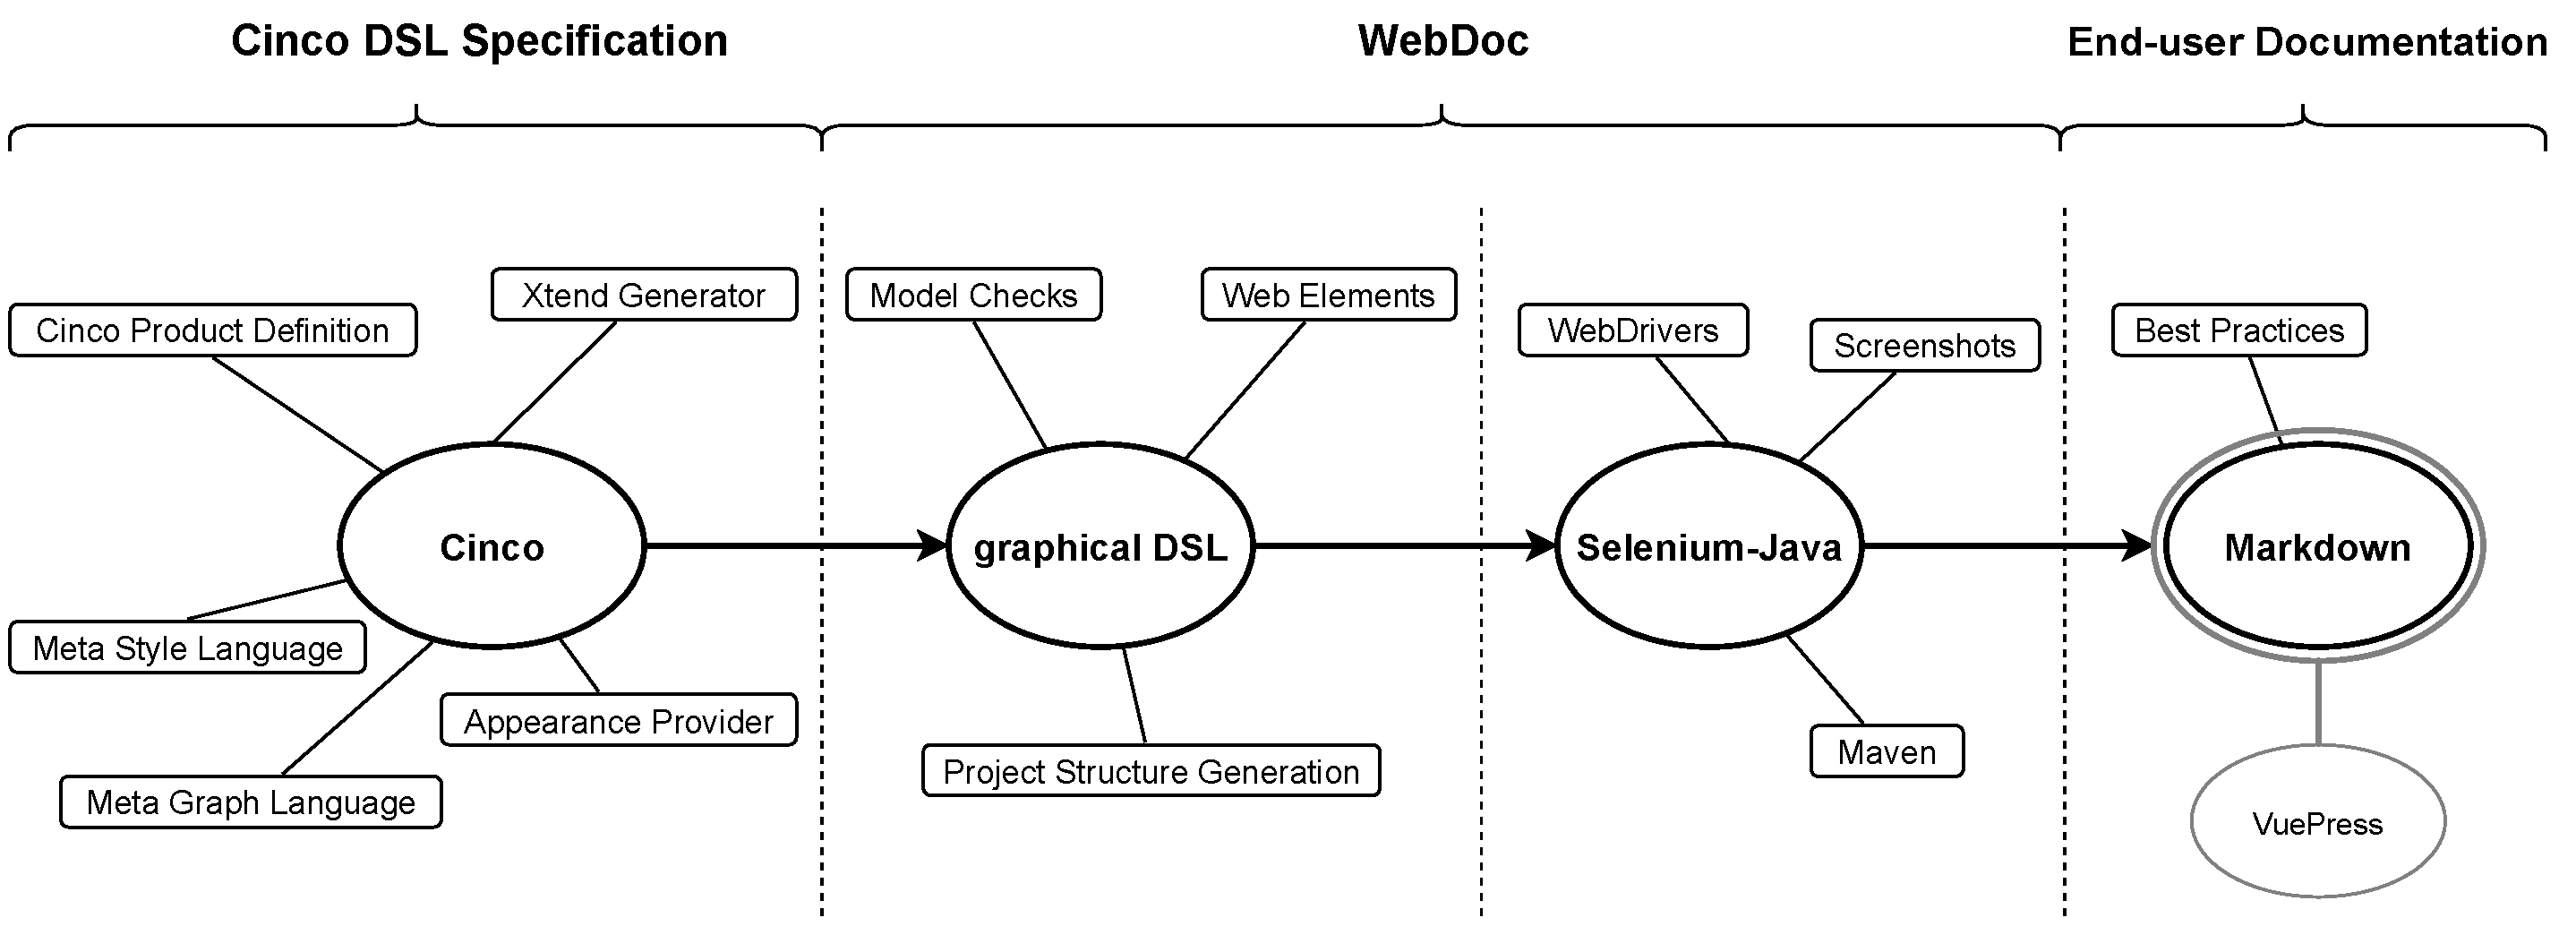
\includegraphics[width=\textwidth]{WebDocDevelopment-all.pdf}
    \caption{Development path of the end user documentation}
    \label{fig:procWorkflow}
\end{figure}

This chapter introduces the key concepts that were used for achieving the objectives assigned for this thesis. We begin by considering the format of our end user documentation as recommended by known standards (from the ISO/IEC\footnote{\gls{iso} and \gls{iec}} and IEEE\footnote{\gls{ieee}}) and the technologies available to assist us in completing this task. The \textsc{Cinco} Meta Tooling Suite will next be used to introduce the principles of model-driven programming, as well as introduce the metalanguages that ground our graphical models and quickly describe the product generated from those models. Finally, we elude the overall generation process to achieving our goal (see figure \ref{fig:procWorkflow}).

\pagebreak

\section{End User Documentation}\label{sec:endUserDoc}

The value of a good software product, in fact, of any product destined for the consumer, is determined by how effective the end user can learn to use and work with it. Hence, putting a great effort to generate and manage sound, well-structured, and well-written documentation is as essential as the development of the product itself~\cite{ISO-IEC-IEEE}. 

End user documentation aims to provide application end users with the knowledge to interact with the software appropriately. It is an integral aspect of the development process and serves as a link between the product creator and the end user~\cite{9238529}. By increasing the structure and usability of the information supplied to end users, the developer not only reduces the number of support calls but also improves the product's and the developing company's reputation~\cite{ieee5712775}.

In this section we will describe the main characteristics of an end user documentation, focusing on the standards established by the ISO/IEC and the IEEE~\cite{ieee5712775, ISO-IEC-IEEE}, before writing about the specifics of documenting Web applications by giving an example of a documented Web application. We will also present the technologies used currently for creating and managing such documentation. Our main goal is to produce an entire end user documentation page from a graphical model. It is worth noting at this stage that the type of documentation to be created will depend on how the documentation designer lays out the model. Meaning that the model could be designed to represent technical documentation -- requiring deep knowledge of the application documented -- or it could also be structured to produce documentation for simple end users with no technical knowledge at all of the underlying Web application~\cite{ieee6081814}.


\subsection{Documentation Characteristics}\label{sec:char}

Since our focus is primarily on Web applications, we will be documenting the \glsentryfull{ui}, which is composed of Web elements (such as buttons, navigation links, checkboxes) the user can interact with. This settles implicitly the type of documentation we aim to create: a step-by-step guide for navigating UI to reach the expected result. Nonetheless, the ISO/IEC/IEEE Standard 26511:2012~\cite{ieee6170926} mandates, i.e.,~that completeness and accuracy should be of the utmost importance when designing the end user documentation.

A good documentation should respond to three essential questions: \textit{why} the application has been developed, meaning the problem the application intends to solve, \textit{what} is the end user supposed to do to get to the solution quickly and efficiently and \textit{how} it is achieved~\cite{ISO-IEC-IEEE}. Information gathering is a task we leave to the information manager. However, the last question is better answered by providing visual help as screen captures or any illustration that fastens the understanding of the documentation. 

As previously stated, we plan to document Web applications from the perspective of the application's end user. That means that the documentation developer must consider the product's audience, and identifying the core jobs and activities performed by the ordinary users should be an essential element of the design process~\cite{ISO-IEC-IEEE}. Thus, our solution puts the developer in charge of the production of a detailed and comprehensive documentation.

\subsection{Documentation Software Tools}

Choosing the format to bring the documentation to the end user is as important as the rest of the milestones of the planning process. A poor decision in this area might limit the documentation's ability to reach many consumers, rendering it useless. Choosing technologies that have already received widespread adoption is a wise move. That ensures a broader reach and prior knowledge within the same audience:

\subsubsection{Markdown}\label{sec:MD}

Markdown is a lightweight markup language created by John Gruber\footnote{John Gruber's official project website \url{https://daringfireball.net/projects/Markdown/}} in 2004. Since then, it has established itself as one of the world's most popular markup language~\cite{Markdown}. Gruber states on his webpage that Markdown is comprised of formatting syntaxes that can be applied to plain-text files and optionally a converter to other markup languages files like \gls{html}. Hypertext means the link that connects Web pages, either within the same website or between different websites~\cite{mozillaMDN}. On the Mozilla Developer Network website\footnote{MDN: \url{https://developer.mozilla.org/en-US/docs/Web/HTML}}, \gls*{html} is described as the fundamental building block of any Web page that uses markup syntax to annotate text, images, and other content for display in a Web browser.

Markdown's popularity makes it an excellent choice for our project since the description of the UI is first made as plain-text and then transformed to a rich-text format using markup syntax as depicted below. Moreover, Markdown files can be opened and edited with any kind of text editor available. Finally, a tremendous amount of documentation about Markdown syntax is available online for the interested reader to get started.

\begin{figure}[h]
    \centering
    \includegraphics[width=\textwidth]{Markdown.pdf}
    \caption{Plain-text transformation with Markdown}
    \label{fig:Markdown}
\end{figure}

A plethora of applications exists for transforming Markdown files into HTML files to be rendered in a Web browser application -- such as MacDown~\footnote[1]{MacDowns: \url{https://macdown.uranusjr.com/}} for Mac users, ghostwriter~\footnote[2]{Ghostwriters: \url{https://wereturtle.github.io/ghostwriter/}} for Windows and Linux, or an online tool like Dillinger~\footnote[3]{Dillinger: \url{https://dillinger.io/}}. Even so, we choose to work with one framework that has also established itself throughout the developer community and that works especially very well with Markdown files: VuePress.

\subsubsection{VuePress}\label{sec:VP}

VuePress is a minimalistic VueJS-powered static website generator. VueJS~\cite{vuepress} is an open-source JavaScript framework designed by Evan You\footnote[4]{Eva You's website \url{https://evanyou.me/}}. It is minimalistic because it only takes a few lines of configuration and two commands to create and launch a static website. It is resilient and up-to-date since it is open-source software and is maintained by a large community of contributors.

By respecting the VuePress conventional folder structure, it can explore folders, get Markdown files, and convert them to HTML files. The default appearance of the generated website is defined by a customizable configuration file included in the project folders. By simply adding certain configuration elements, one may create, i.e.~a sidebar menu and a navigation bar. VuePress produces a static website by building hyperlinks between HTML files in the project folder hierarchy. That means that subfolder Markdown (or HTML) files are rendered as menu items on the folder's HTML page. A server-rendered website with a live reload mechanism is constructed and launched after inputting the correct command. Thus, every modification to the Markdown files is immediately visible on the website. The final step is to create the website that will be saved in a particular folder and exported to any other website.

We will use VuePress to statically launch the end user documentation as a website, relieving the developer of configuring the server. The principal task remaining is, therefore, to create a solid documentation model.


\section{Core Principles of Model-Driven Development}\label{sec:mdd}

This section lays down the fundamentals of the \gls{mdd} -- also referred to as \gls{mdsd}~\cite{fowler} --  using the \textsc{Cinco} SCCE Meta Tooling Framework, as well as the steps necessary to get up and running with the framework. The term MDD refers to a development paradigm where the functionalities of the software are first specified as models, from which then executable code can be automatically generated. A DSL close to the problem domain is needed to create models to represent the software system. Application domain experts know the application structure, which they represent in the form of models. Domain experts and application programmers must agree on how the specification language determines the syntax and semantic of the model elements.

The core principles of MDD are that software development is accelerated by providing a simple but efficient abstraction of the software structure as a model. Those model abstractions, representing real-world objects, are transposed through a series of model-to-model or model-to-code transformations~\cite{stahl_et_al}. Our work is to utilize the DSL provided by the \textsc{Cinco} framework and design our graphical DSL to generate a functioning \gls*{selenium}-Java application (Selenium is a suite of application tools for automating Web browsers) that takes screenshots of the different Web application states.

As opposed to the standard development method, applying a graphical model to layout the different user sequences allows even non-programmer (here the domain expert with much more expertise on how to design excellent software documentation) to document the features offered by the Web application. Nonetheless, the programmer has the tasks -- in collaboration with the domain expert -- to specify the meaning of each model element for the code generation process. 

When applied correctly, the result of the model-driven development process is a tailored application to a domain. That reflects one of the main advantages of MDD: the accuracy of directly targeting the specific problem~\cite{brambilla2017model}. Besides, it is still possible to change the DSL to adapt to the new challenges emerging during the development process. That can be iterated until the specification reaches preciseness wanted to solve the problem.

\section{Domain-Specific Language}\label{sec:DSL}

A \glsentryfull{dsl}, as described before, is a language adapted to a specific development domain. In~\cite{Naujokat2018} a succinct analogy to \glsplural*{dsl} is given by saying that it is comparable to a tool specially crafted only for one specific task as opposed to general programming languages, which can be seen as tools for multiple different tasks. Just as one would start with a blueprint to construct a mechanical tool, designing as DSL required similar steps. One must conceptually layout the behavior and eventually -- in case it is a graphical language we seek to design -- the look of each element that can be used in our DSL.

Blueprinting our DSL is equivalent to defining a metalanguage or meta-DSL tool. \textit{Meta} literally means \textit{situated behind or beyond}\cite{merriam}. So, metalanguage is a descriptive language that comes before and describes the meaning (semantic) and the relationship between the objects of our target language. Put differently, the meta-DSL is the abstract syntax, and the DSL concrete syntax is the result. It is feasible to work our way up the meta-definition modeling hierarchy until we reach a self-referencing language, as is the case for the \gls{uml}.

In our case, we want a graphical language for creating models that represent the different parts of a Web application and how the end user can interact with them. The metalanguage to our graphical DSL is provided by the \textsc{Cinco} SCCE Meta Tooling Suite. It comprises the \gls{mgl}, the \gls{msl} and the \gls{cpd}. All have been constructed using Xtext~\cite{bettini2016implementing}, a language Workbench for writing textual \glspl*{dsl}~\cite{naujokat-diss}. The next section explains these concepts in detail.

\section{\textsc{Cinco SCCE} Meta Tooling Framework}\label{sec:cincoFW}


The \textsc{Cinco} Framework is a generator-driven development environment for domain-specific graphical modeling tools~\cite{Cinco}. The chair of programming systems currently develops it at the Technical University of Dortmund amongst many other projects of the SCCE Group \footnote[1]{\url{https://www.scce.info/}}, which aims at allowing the application-domain experts, rather than programming experts, to take charge of the development tasks~\cite{scce}. One of the great features of this framework is that it allows us to generate an entire editor application with just one click from a simple textual specification language -- the MGL mentioned in the previous section. 

The MGL, together with the MSL, form the metamodel from which \textsc{Cinco} generates a ready-to-run modeling tool called \textsc{Cinco} product. The MSL defines the look for each graph element, the font, and the color of the text displayed in the graphical model~\cite{naujokat-diss}. The created metamodel is based on Ecore, the metamodeling language of the \gls{emf}. Furthermore, the Graphiti framework generates the corresponding graphical model editor. Additionally, there is a button to trigger code generation in the created editor. Chapter~\ref{ch:CP} is devoted to our \textsc{Cinco} product (the editor application), in particular section~\ref{sec:GenProcess} gives an in-depth explanation of the generation process.

\begin{figure}[h]
    \centering
    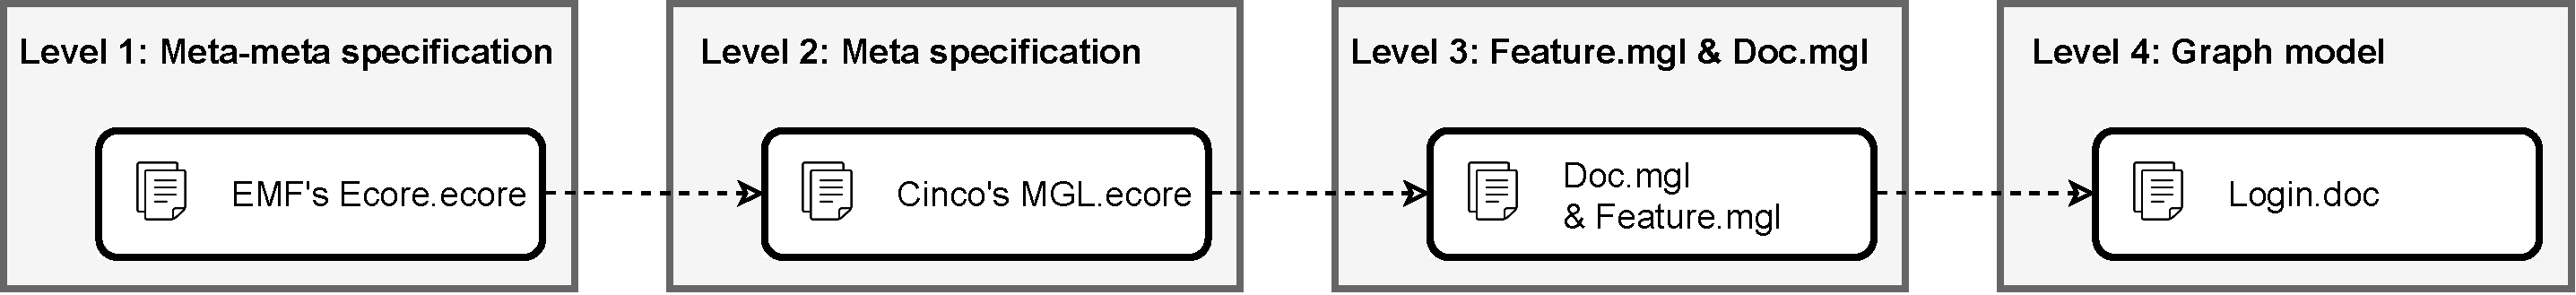
\includegraphics[width=\textwidth]{SpecsHierarchy.pdf}
    \caption{Hierarchy of our graphical DSL specification}
    \label{fig:modeling-hierachy}
\end{figure}

The full generation process of a graphical modeling tool (of a \textsc{Cinco} Product Application) comprises four essential (meta) levels~\cite{Naujokat2018} as shown in figure \ref{fig:modeling-hierachy}. The first level, associated with Eclipse Developer's role, is where the Ecore.ecore and GraphitiDiagram.ecore metamodel are developed. The second level is where \textsc{Cinco} Developers of the Chair 5 for Programming Systems developed the MGL.ecore using the metamodel from the first level. That second-level metamodel, in turn, becomes metamodel of the third specification level. The level where the \textsc{Cinco} Product Developer operates and where this thesis comes in, see fig.~\ref{fig:modeling-hierachy}. That means the Eclipse Developers are now at the meta-meta level, the \textsc{Cinco} Developers at metalevel of the specification elaborated in this work. For the remainder of the chapters, we will be focusing on the third and fourth specification levels because the fourth level, for example, is where the \textsc{Cinco} Product Users use the generated graphical editor to create the domain-specific models.

\subsection{Meta Graph Language}\label{sec:MGL}

The \gls*{mgl} sketches the behavior, the constraints and gathers all the graphical components that will constitute the model elements that come into use in every graph diagram created in the modeling tool. This is where we start developing our editor application: the main elements that can be define in a MGL are \textbf{nodes}, \textbf{containers} and \textbf{edges} as illustrated in listing~\ref{featMGL}.

The main graph model, the \lstinline{FeatureGraphModel}, is the one containing all the features of the Web application we want to be documented. For instance, our  Web application provides the login feature as the starting point. After successfully logging in and accessing the dashboard, task lists can be created or deleted; tasks can be added to or removed from them. The graph diagram can be assigned a name and description. We specified \lstinline{.feat} (short for feature) as model extension. Moreover, since the login feature, i.e.,~requires a series of user actions to be performed, the FeatureGraphModel contains another graph model type, where those sequences of actions are modeled: the \lstinline{DocGraphModel}. The DocGraphModel contains the meta specification of all the frequently used Web elements we want to use in our graph models. It also comprises sectioning elements to structure the diagram and edges to connect them. The listing below shows an excerpt from the concrete FeatureGraphModel implementation.

\begin{lstlisting}[language=MGL, caption={Excerpt from the feature.mgl, meta-specification of the FeatureGraphModel}, label=docMGL, escapechar=|]
    graphModel FeatureGraphModel { |\label{line:modelStart}|
        iconPath "icons/16/feature_16.png"
        diagramExtension "feat"
        containableElements(FeatureContainer,DocNode[1,*])
        attr EString as modelName := "New Feature"
        attr EString as description := "New Description"
    }|\label{line:modelEnd}|
    
    container FeatureContainer { |\label{line:featCont}|
        style featureContainer("${title}")
        containableElements(Start[1,1], Stop[1,1],DocNode[1,*])|\label{line:multiplicity}|
        attr EString as title := "New Feature"
        @multiLine
        attr EString as documentation := "This feature is about ..."
    }
    
    node DocNode{ |\label{line:docNode}|
        style docNode("${mgl.modelName}")
        prime docMgl::DocGraphModel as mgl |\label{line:prime}|
        attr EBoolean as createScreenshots := true
        incomingEdges (Edge[1,1])
        outgoingEdges (Edge[1,1])
    }
\end{lstlisting}

It can be seen from listing \ref{docMGL} that we define a container element to hold the DocGraphModel instances (see lines~\ref{line:featCont} and \ref{line:docNode}). To integrate a whole DocGraphModel inside a FeatureGraphModel, we used the so-called \textit{PrimeReference}, which is a \textsc{Cinco} feature that allows referencing another model by only one attribute of a node or container~\cite{Cinco}. It is applied by adding the keyword \lstinline[language=MGL]{prime}, as we did in line~~\ref{line:featCont}. By doing so, we can drag and drop a DocGraphModel diagram into a FeatureGraphModel diagram to incorporate it.

As for the DocGraphModel, we specified four categories of model elements that are used while designing the diagram: the most important ones, the Web elements, represent the UI element the user can interact with. Then we have the Selenium action nodes, which perform specific actions to drive the Web browser using the Selenium WebDriver. Those are, i.e., the Navigation node to change from one Web page to another and the Screenshot node to capture the current application state as an image. Finally, we have the semantic element \lstinline{Comment} to give a descriptive text to the screenshots and the basic elements (start and end as well as the section node), which help structure the user sequence graph.

\begin{lstlisting}[language=MGL, caption={Excerpt from the Doc.mgl, meta-specification of the DocGraphModel}, label=featMGL, escapechar=|]
    graphModel DocGraphModel {
        iconPath "icons/16/sequence_16.png"
        diagramExtension "doc"
        containableElements(*)
        attr EString as modelName := "UserSequence"
        @multiLine
        attr EString as documenation := "Lorem ipsum dolor et si met"
    }
    
    node Screenshot {
        style screenshotNode
        incomingEdges (Transition[1,1], Anchor[1,*])
        outgoingEdges (Transition[1,*])
        attr EString as pictureName
        attr Comment as description
    }

    node Input extends WebElement {
        style inputNode("Input: ${content}")
        attr EString as content
        incomingEdges (Transition[0,*])
        outgoingEdges (Transition[0,*])
    }
\end{lstlisting}

For demonstration purposes, we kept our example listings short. An exhaustive list of all the usable elements and annotations can be found on the \textsc{Cinco}'s documentation page\footnote[1]{Wiki page : \url{https://gitlab.com/scce/cinco/-/wikis/Cinco-Product-Specification}}.

\subsection{Meta Style Language}\label{sec:MSL}

The appearance of all the elements defined in the MGL is laid down using the textual \glsentryfull{msl}. As explained in~\cite{gitlabcinco}, three essential elements constitute the design of a MSL model, namely: \textbf{appearance}, \textbf{nodeStyle} and the \textbf{edgeStyle}.

Each nodeStyle specification makes use of an appearance element, which in fact determines the attributes like background color, the thickness of the drawn lines and so on (see listing~\ref{docStyle}). The nodeStyle is hierarchically composed of a shape that can be given a \lstinline[language=MGL]{size}, \lstinline[language=MGL]{position} and a \lstinline[language=MGL]{text} element with a \lstinline[language=MGL]{value} attribute that takes a (format) string (line~\ref{line:strFormat}) that will be display in the graphical model. We can say that it is left to the \textsc{Cinco} product developer's imagination to style the elements as seen fit.

\begin{lstlisting}[language=MGL, caption={Excerpt from feature.style to be applied to feature.mgl}, label=docStyle, escapechar=|, name=docMSL]
    nodeStyle featureContainer(1) {
        rectangle {
            appearance extends default { |\label{line:inheritance}|
                background (246,245,244)
            }
            size (300,75)
            text {
                appearance {
                    font("Sans", BOLD, 10)
                }
                position (LEFT 5, TOP 5)
                value "%s" |\label{line:strFormat}|
            }
        }
    }
\end{lstlisting}

It is also worth mentioning that the concept of inheritance from the \gls*{oop} can be applied between metamodel elements of the same type. Thus, avoiding repetitive definitions of the same attributes within multiple different elements and allowing some elements to extend the properties of the parent elements. For example, we see in line~\ref{line:inheritance} that the \lstinline{featureContainer} appearance extends the default one and at the same time redefines the background color.

\subsection{Cinco Product Definition}\label{sec:CPD}

In the \glsentryfull{cpd} is where it all comes together. Herein, the \textsc{Cinco} Product Developer must provide key information like the \textsc{Cinco} product name, at least one or more MGL files to be included in the generation process. Optionally, one can set up a splash screen with branding images, add descriptive text about the application and specify plugins and features~\cite{gitlabcinco}.
The listing below gives an insight into the CPD specification language.

\begin{lstlisting}[language=MGL, caption={UserDocumentationTool.cpd}]
    CincoProduct UserDocumentationTool {
        mgl "model/Feature.mgl"
        mgl "model/Doc.mgl"
        
        splashScreen "branding/splash.bmp" {
            progressBar (37,268,190,10)
            progressMessage (37,280,190,18)
        }
    
        image16 "branding/Icon16_dark.png"
        image32 "branding/Icon32.png"
        image48 "branding/Icon48.png"
        image64 "branding/Icon64.png"
        image128 "branding/Icon128.png"
        linuxIcon "branding/Icon512.xpm"
	
        about {
            text "WebDoc is a DSL-driven generator of end user documentation for Web applications. It is a bachelor thesis project developed with the Cinco SCCE Meta Tooling Suite ( http://cinco.scce.info )."
        }

        plugins {
            info.scce.cinco.product.userdocumentation.edit,
            info.scce.cinco.product.userdocumentation.editor
        }
    }
\end{lstlisting}

\subsection{Xtend Generators}\label{sec:GEN}

We need to create two different application folder structures from our model diagrams for our application documentation: the first is the Selenium-Java application, which replays the modeled user action sequences and takes screenshots as laid out by the designer. It follows the specific Maven project structure, for which we applied the rule of convention over configuration as recommended on the Maven Apache \footnote[1]{\url{https://www.apache.org/}} website and added Selenium as a dependency. The second project structure we generate following convention is the VuePress project that comprises the Markdown files containing all semantic text the documentation developer specified as description or comment in the model elements. We create the modeled end user documentation by following each sequence beginning from the start node to the end node and constructing a cohesive documentation text.

This generation approach utilizes the Java's and Xtend's text templating feature, which is based on the generation pattern used in the \glsentryfull{jabc}~\cite{model-driver-dev_jABC,jabc-home}. In fact, many generator classes in our example project implement and extends interfaces from the generator runtime and template package of the jABC \textsc{Cinco} meta plugin.

Additionally, other template classes are implemented to create the configuration files, the application class files, and project files. In chapter~\ref{ch:intro} section~\ref{sec:objectives} we provided a link to the GitHub repository, where the complete application code can be found. In the following chapters, we show the output of the generator and feature classes while introducing our application as an ongoing example.

\section{Tasks management Web application -- TODO-App}\label{sec:todoApp}

The TODO-App is a Web application entirely generated with the \gls{dime}~\cite{bosselmann-et_al}, a development environment for creating Web applications. DyWA stands for dynamic Web applications; it is the container used to host the generated application. While the modeling and the code generation happen in DIME, DyWA provides support for the product deployment phase, constitutes the runtime environment, and manages the data persistence~\cite{bosselmann-et_al}.

\begin{figure}[h]
    \centering
    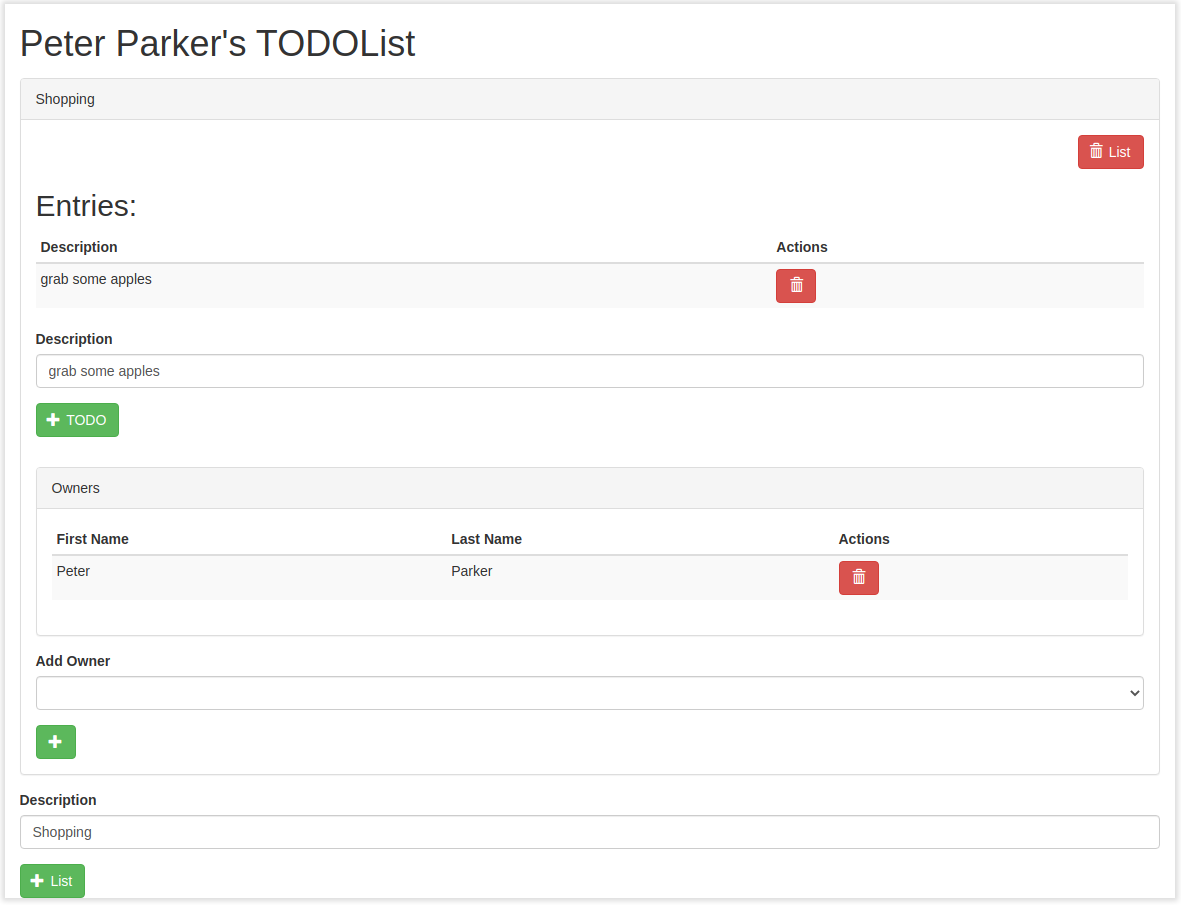
\includegraphics[width=0.8\textwidth]{todoApp.png}
    \caption{Impression of the TODO-App Web interface}
    \label{fig:todoApp}
\end{figure}

The TODO-App is an application that helps manage lists of tasks to be done. It provides a logged-in user with the possibility to create such lists, add various tasks to them, and after their completion, remove them~\cite{bosselmann-et_al}. Users also can add co-owners, which are other existing users, that can manage that respective list with them. The application is launched in development mode, meaning that it is accessible via a local Web address (\lstinline{http://localhost:8080}) from the host it has been started in. The TODO-App is ideal for demonstration purposes since it presents all the Web elements necessary to a Web application interface, as depicted in figure \ref{fig:todoApp}.

DIME's model-driven development concept was our starting point. Thus, the graphical elements meta specification focuses on specifying elements that represent the graphical user interface (GUI) and those that implement processes. The latter are elements whose semantic implementation will direct the Web browser to recreate the procedures necessary to construct the intended documentation. However, in our scenario, the concept of data permanence is not required. Furthermore, even though our concept grounds on DIME, it does not mean that our application is only for DIME-generated Web apps. In this respect, any navigable Web application can be modeled with our editor and thus documented.